\chapter{Word order in the investigated languages}\label{chap:key:3}

The word order in the three languages under investigation -- Turkish, Kurmanji Kurdish, and German -- is SOV. However, each language also allows certain constituents to appear in the post-predicate position. The use of this position is influenced by different factors: information structure in Turkish, predicate semantics in Kurmanji, and syntactic structure in German. At the same time, there are overlaps in the factors that govern the placement of constituents in the post-predicate position.

Importantly, constituents in the post-predicate position can be clausal and non-clausal. This study focuses specifically on non-clausal post-predicate constituents. The rationale behind this decision is that including clausal constituents would involve the discussion of clause-combining, which is a different, although definitely related, topic.

This chapter provides a detailed overview of word order in the three languages, with a particular focus on non-clausal post-predicate constituents. Additionally, relevant studies on word order in these languages in contact situations are summarized.

\section{Word order in Turkish} \label{sec:key:3.1}

Turkish is considered to have a relatively free word order, with the basic word order being SOV (\citealt{Erguvanli1984}: 5, \citealt{GokselKerslake2004}: 343-346). This implies that even though word order variation is possible, there are certain instances where the word order must remain fixed. One such case occurs when noun phrases lack case marking and there are no semantic cues to distinguish their grammatical roles, as illustrated in the following examples (\citealt{Erguvanli1984}: 5):

\ea\label{ex:key:1} Turkish (\citealt{Erguvanli1984}: 5)\\
\gll Mutluluk   huzur    getir-ir.\\
happiness  serenity  bring\textsc{-aor.3\textsc{sg}}\\
\glt ‘Happiness brings serenity.’
  \z

\ea%2
  \label{ex:key:2} Turkish (\citealt{Erguvanli1984}: 5)\\
\gll Huzur     mutluluk   getir-ir.\\
serenity          happiness         bring\textsc{-aor.3\textsc{sg}}\\
\glt ‘Serenity brings happiness.’
  \z

Variation in word order in Turkish is employed to serve pragmatic purposes, such as signaling topics and distinguishing between old and new information (\citealt{Erku1983}, \citealt{Erguvanli1984}: 44-50, \citealt{Issever2003}). Thus, word order in Turkish is strongly governed by information structure, where topicalized information appears sentence-initially, new information occurs immediately before the verb, and backgrounded information can be placed post-verbally (\citealt{Erku1983}, \citealt{Erguvanli1984}, \citealt{Hoffman1995}). For instance, the example \REF{ex:key:3a} below has pragmatically neutral unmarked order, whereas examples (3b--f) are pragmatically marked.



\ea\label{ex:key:3} Turkish, self-constructed \\
\ea\label{ex:key:3a}
\gll Murat     araba-yı   sat-tı.\\
Murat    car-\textsc{acc}  sell-\textsc{pst}.3\textsc{sg}\\
\glt ‘Murat sold the car.’\jambox*{SOV}

\ex\label{ex:key:3b}
\gll Araba-yı  Murat    sat-tı.\\
car-\textsc{acc}  Murat    sell-\textsc{pst}.3\textsc{sg}\\
\glt ‘It is Murat who sold the car.’\jambox*{OSV}

\ex\label{ex:key:3c}
\gll Murat    sat-tı    araba-yı.\\
Murat    sell-\textsc{pst}.3\textsc{sg}  car-\textsc{acc}\\
\glt ‘Murat did sell the car.’\jambox*{SVO}

\ex\label{ex:key:3d}
\gll Araba-yı   sat-tı     Murat.\\
car-\textsc{acc}  sell-\textsc{pst}.3\textsc{sg} Murat\\
\glt ‘It is the car that Murat sold.’\jambox*{OVS}

\ex\label{ex:key:3e}
\gll Sat-tı     Murat     araba-yı.\\
sell-\textsc{pst}.3\textsc{sg}  Murat    car-\textsc{acc}\\
\glt ‘Sell is what Murat did to the car.’\jambox*{VSO}

\ex\label{ex:key:3f} 
\gll Sat-tı     araba-yı   Murat.\\
sell-\textsc{pst}.3\textsc{sg}  car-\textsc{acc}  Murat\\
\glt ‘Sold the car is what Murat did.’\jambox*{VOS}
\z
\z


As shown in the examples above, scrambling in Turkish can result in certain constituents being placed in the post-predicate position, typically to background them. This backgrounding occurs under specific conditions: when the elements are discourse-predictable (i.e., previously mentioned or easily inferable from context) or supplementary (providing less crucial information for the listener) (\citealt{Erguvanli1984}). Consequently, information in the post-predicate position can often be omitted \citep{Hoffman1995}. Moreover, elements in this position are never stressed, as indicated by their flat and low intonation contour \citep{Kornfilt1997}.

Post-predicate constituents in Turkish may be of several types: noun phrases (NPs), adverbs, connectors, discourse markers, as well as subordinate clauses (\citealt{AkanHartmann2019}, \citealt{Erguvanli1984}, \citealt{Kornfilt1998}, \citealt{GokselKerslake2004}). Furthermore, there is no restriction on the number of constituents that occur after the predicate, and the order of the constituents after the predicate appears to be more flexible compared to the order of constituents in the pre-predicate position \citep{Skopeteas2015}. However, certain constituents are always placed in the post-predicate position. These are, for example, discourse markers that emphasize the preceding verb or the whole utterance but do not receive stress themselves. Thus, in example \REF{ex:key:4}, the discourse marker \textit{ki} emphasizes the whole utterance and follows the verb immediately.


\ea%4 
  \label{ex:key:4} Turkish, self-constructed \\
  \gll Ben  bun-u    yap-ma-dı-m    ki.\\
 I  this-\textsc{acc}  do-\textsc{neg-pst-1sg}  \textsc{dm}\\
 \glt  ‘But I haven’t done this!’ 
  \z

Nevertheless, there are restrictions on the types of constituents that may be placed in the post-predicate position (\citealt{Erguvanli1984}, \citealt{GokselKerslake2004}). Focus constituents, contrastive elements, new concepts, and unactivated topics do not appear in the post-predicate position in Turkish (\citealt{Erguvanli1984}, \citealt{Schroeder1995}). For example, no question constituent can be placed after the predicate because they are always focused.


\ea \label{ex:key:5} Turkish, self-constructed \\
\ea[]{\label{ex:key:5a}
   \gll Anahtar-ı san-a kim ver-di? \\
        key\textsc{-acc} you-\textsc{dat} who give-\textsc{pst.3\textsc{sg}}\\
   \glt ‘Who gave you the keys?’
}
\ex[*]{\label{ex:key:5b} 
   \gll Anahtar-ı san-a ver-di kim?\\
        key\textsc{-acc} you-\textsc{dat} give-\textsc{pst.3\textsc{sg}} who\\
        \glt Intended: ‘Who gave you the keys?’
} 
\z
\z


In example \REF{ex:key:5a}, the question word \textit{kim} ‘who’ appears immediately before the verb due to its focus. In contrast, example \REF{ex:key:5b} would be considered noncanonical, as placing the question word in the post-predicate position would background it -- an impossible structure in interrogative sentences.

Another restriction is that indefinite NPs cannot occur in the post-predicate position because they usually contain new information (\citealt{Erguvanli1984}). Consider the following examples:

\ea%6
  \label{ex:key:6}  Turkish, self-constructed \\
\ea[]{\label{ex:key:6a}
 \gll Dün    bir  kitap  al-dı-m \\
 yesterday  \textsc{art}  book  buy-\textsc{pst-1sg}\\
\glt ‘Yesterday I bought a book.’ 
 }
\ex[*]{\label{ex:key:6b}
\gll Dün    al-dı-m   bir  kitap\\
 yesterday  buy-\textsc{pst-1sg}  \textsc{art}  book \\
}
\z
\z

Thus, in example \REF{ex:key:6a}, the indefinite NP \textit{bir kitap} ‘a book’ is placed in the immediate preverbal position because in this sentence it is focused, whereas example \REF{ex:key:6b} with \textit{bir kitap} ‘a book’ in the post-predicate position would be considered noncanonical.

Nevertheless, under some conditions, new information can occur also in the post-predicate position. These instances are usually afterthoughts. An afterthought is a prosodically and syntactically independent unit, whose discourse function is to repair an unclear reference (\citealt{Benz2008}). \citet{Erguvanli1984} notes that in Turkish there is usually a slight pause between a predicate and an afterthought. Another indicator of an afterthought in Turkish is the word \textit{şey} `thing' positioned before the verb, serving as a placeholder for the material that appears as an afterthought. An example for this comes from \citet[51]{Erguvanli1984}:


\ea%7
  \label{ex:key:7} Turkish (\citealt{Erguvanli1984}: 51)\\
\gll Koca-sı    şey-de    çalış-ıyor    fabrika-da \\
 husband-\textsc{poss}.3\textsc{sg}  thing-\textsc{loc}  work-\textsc{prs}.3\textsc{sg}    factory-\textsc{loc}\\
\glt ‘Her husband works at-the-what-do-you-call-it, at the factory.’
  \z

Thus, in the example \REF{ex:key:7}, \textit{şey} signals that the location is being added as an afterthought, with the actual referent (\textit{fabrikada} ‘at the factory’) provided postverbally.

Furthermore, when the whole utterance is new, there may be post-predicate elements that are backgrounded in relation to the whole utterance. Besides, when there are several new constituents, the “less important” one can be placed in the post-predicate position. This often occurs when there is no intention to bring attention or emphasis to that particular constituent (\citealt{Kilicaslan2004}, \citealt{DogruozBackus2007}, \citealt{AkanHartmann2019}, \citealt{Issever2019}). An example for this is provided in \citet[204]{DogruozBackus2007}:


\ea%8
  \label{ex:key:8} Turkish (\citealt{DogruozBackus2007}: 204)\\
       Seza:
       \gll Türkçe-yi nerde öğren-di-n? \\
  Turkish-\textsc{acc} where learn-\textsc{pst}-\textsc{2sg}\\
 \glt  ‘Where did you learn Turkish?’

Seren:
\gll  O da aile-m-den sonra ilkokul-da hep Türk okul-u-na gid-il-di hafta-da bi defa.\\
  that \textsc{dm} family-\textsc{poss}.\textsc{1sg}-\textsc{abl} then primary.school-\textsc{loc} always  Turkish school-\textsc{poss}.\textsc{3sg}-\textsc{dat} go-\textsc{pass}-\textsc{pst} week-\textsc{loc} one time. \\
\glt ‘That is also from family, then we went to Turkish school during primary school once a week.’
  \z

In Example \REF{ex:key:8}, the postverbal element \textit{hafta-da bi defa} ‘once a week’ conveys new information and would therefore be expected to appear in the preverbal area. However, \citet{DogruozBackus2007} show that monolingually raised Turkish speakers in Turkey do not treat this as a violation, suggesting that the ban on postverbal focused elements is not as strict as previously assumed. Moreover, the authors show that similar examples can also be found in Turkish spoken in Turkey.

\subsection{The effect of formality and mode on the use of the post-predicate position} \label{sec:key:3.1.1}

Importantly, while post-predicate placement is not inherently noncanonical in Turkish, its usage is influenced by factors such as formality and mode. Sentences with post-predicate constituents are found in both written and spoken Turkish (\citealt{Antonova-unlu2015}). However, their usage is significantly more common in unplanned spoken discourse than in structured written texts (\citealt{Schroeder1995, Schroeder2002}, \citealt{Erdal1999}). This is because spoken discourse is typically spontaneous, often including afterthoughts and self-corrections. The post-predicate position aids listeners in keeping track of topic development and the deictic context in which the predication occurs \citep{Schroeder1995}.

Furthermore, \citet{Erguvanli1984} emphasizes that formality significantly influences the use of post-predicate structures. In highly formal styles of Turkish, such as legal documents and news items—whether written in newspapers and journals or broadcast on radio and TV—these structures are exceedingly rare. This rarity stems from normative pressures on the use of post-predicate structures in the formal language. A key factor behind this restriction is the politicized nature of the Turkish language in Turkey, any deviation from the standard sentence structure is often perceived as a foreign influence and met with resistance (\citealt{Erdal1999}, \citealt{KucukEtAl2017}).

In summary, word order in Turkish, and particularly the employment of the post-predicate position, is driven by the information structural requirements. This position is reserved for background information, hence, focused and new information is generally not allowed in this position. Moreover, mode (spoken vs. written) and formality (formal vs. informal) play a role in the employment of the post-predicate position. This position is characteristic of informal, unplanned spoken discourse, whereas its use is constrained by normative rules in formal settings.

\section[Post-predicate position in {Turkish} in language contact situations]{Studies on the post-predicate position in {Turkish} in language contact situations}\label{sec:key:3.2}

The use of the post-predicate position in Turkish has captured the attention of researchers, both in monolingual and multilingual contexts. While previous studies generally confirm that Turkish predominantly follows SOV word order, the reported proportions of pre- vs. post-predicate structures vary significantly across different datasets.

\largerpage
For instance, \citet{Saginsimsek2016} analyzed the speech of monolingual children in Turkey aged 2 to 6 and found that the frequency of post-predicate structures increases with age, rising from 15.9\% in 2-year-olds to 27.1\% in 5- to 6-year-olds. In another study, \citet{Antonova-unlu2015} examined spoken narrations of English-Turkish simultaneous bilingual\footnote{In the referenced studies, Antonova-Ünlü distinguishes between simultaneous and sequential bilingual acquisition. Simultaneous bilingual acquisition occurs when a child is exposed to two languages from birth or within the first week of life. In contrast, sequential bilingual acquisition refers to the situation in which an individual begins exposure to a second language later in life, after having already developed some proficiency in their first language. In \citet{Antonova-unlu2019}, the age of onset for the children learning Turkish ranged from 3 years and 1 month to 6 years and 4 months.} and Turkish monolingual children in Turkey, finding that both groups overwhelmingly favored verb-final word order, with 94--98\% of utterances conforming to this pattern. However, \citet{Antonova-unlu2019} also found that sequential bilingual children, after approximately 2--3 years of exposure to Turkish, used significantly more post-predicate structures than both monolingual and simultaneous bilingual children. Notably, these sequential bilinguals placed indefinite noun phrases or adverbials containing new and/or focused information in the post-predicate position, which deviates from the standard constraints of Turkish. In contrast, all instances of post-predicate use among monolingual and simultaneous bilingual children were rated as canonical. These results indicate that in child language, post-predicate placement is typically canonical for monolingual and simultaneous bilingual children, while sequential bilinguals show more flexibility, placing new or focused information after the predicate.

The occurrence of post-predicate constituents is considerably lower in written language. \citet{Kocak2005}, for example, examined compositions of 9- to 12-year-old children and found that only 4.5\% of their sentences contained postverbal elements. Similarly, Turkish-Dutch bilinguals in the same age group exhibited a comparable pattern, with 4.9\% of their sentences featuring postverbal elements (\citealt{Halitoglu2020}). \citet{TerziyanBackus2023} observed an increase in post-predicate structures even in the written language of monolingual children. However, their study also revealed that Turkish-Dutch bilingual children aged 10-12 used fewer post-predicate structures compared to their monolingual peers.

Research on the use of the post-predicate position in adults yields somewhat different results. For instance, \citet{DogruozBackus2007} examined word order in data from Turkish monolinguals and Dutch-Turkish bilingual adults, finding that 45\% of the utterances in Turkish spoken in the Netherlands and 41\% of those by monolinguals in Turkey contained post-predicate elements. The authors emphasized that the data indicate the information structural requirements for using the post-predicate position remain intact among heritage speakers. Additionally, they found that, under certain conditions, new information can be placed in the post-predicate position in Turkish. Specifically, new elements may appear in the post-predicate position when discourse markers or the particle \textit{şey} ‘thing’ signal that part of the focus will follow, or when the new information in the post-predicate position is less important than another piece of new information presented in the pre-predicate position.

Furthermore, a recent study conducted by \citet{SchroederEtAl2024} examined the use of the post-predicate position using the same methodology as outlined in this study. This research involved Turkish heritage speakers in Germany and the US, as well as monolingual speakers in Turkey. The researchers found no significant differences in the frequency of post-predicate structures among the groups. However, they observed lack of register flexibility among heritage speakers in the US, who used the post-predicate position with nearly equal frequency in both informal and formal communicative situations. In contrast, among monolinguals, this structure was predominantly observed in informal settings and spoken mode.

Another study that examined the post-predicate position in adult speakers is \citet{Haig2024}, who analyzed Turkish as the majority language spoken by Kurmanji-Turkish bilinguals. Importantly, this research builds upon the informal spoken data also investigated in the current study, however, the data were annotated using a different annotation scheme \citep{Iefremenko2021}. Unlike \citet{DogruozBackus2007} and \citet{SchroederEtAl2024}, \citet{Iefremenko2021} found a significantly lower percentage of post-predicate structures, with only about 10\% of the utterances containing a post-predicate element. However, the author also noted considerable individual variation: some speakers had up to 25\% of their utterances featuring post-predicate constituents. Furthermore, the researcher demonstrated that language dominance plays an important role. For instance, Turkish spoken by Kurmanji-Turkish bilinguals in Ankara—where Turkish is the dominant language—showed no signs of convergence with Kurmanji. In contrast, in Erzurum, where Kurmanji is more present, semantic roles and flagging appear to influence the use of the post-predicate position (see \sectref{sec:key:3.3.1} for the definition of \textit{flagging}). These factors, in fact, determine the use of this position in Kurmanji. Thus, it seems that when Kurmanji is more prominent in various spheres of life and the community is larger, changes also occur in the majority language, Turkish.

Changes in word order, particularly concerning the post-predicate position, have also been investigated in other Turkic languages that have been prolonged contact with neighboring languages. For instance, the word order in Karaim shifted from SOV to SVO as a result of contact with Slavic and Baltic languages \citep{Csato2002}. Similarly, the basic word order of Gagauz has changed to (S)VO under the influence of Slavic languages (\citealt{Doerfer1959}, \citealt{Menz1999, Menz2014}, \citealt{Johanson2021}). \citet{Matras_grammatical_Tufan2007-1} report that Macedonian Turkish has shifted toward (S)VO under the influence of Macedonian. Additionally, \citet{Petrou2019} confirmed that in Western Thrace Turkish, the verb is not always placed in the final position, indicating that pragmatic constraints for the employment of the post-predicate position are loosened. Finally, \citet{Keskin2023} conducted a survey across a range of Balkan varieties and found that the frequency of the post-predicate position in the Turkic varieties spoken in the Balkans ranges from 26\% to 75\%. The researcher further asserts that the frequency of the post-predicate position tends to increase as the geographical distance from the Turkish border expands.

These findings suggest that various factors—such as speakers’ age, the duration of contact between languages, the contact language, formality, and mode—can lead to different outcomes in word order changes in Turkish and other Turkic languages. The current study will examine most of these factors, with the exception of speakers’ age.

\section{Word order in Kurmanji}\label{sec:key:3.3}

Northern Kurmanji is a Kurdish language primarily spoken in southeastern Turkey, northwestern and northeastern Iran, northern Iraq, and northern Syria. It belongs to the northwest Iranian branch of the West Iranian languages, which are part of the larger Indo-European language family (\citealt{HaigMatras2002}).

Kurmanji itself comprises several dialects: southeastern dialect (spoken in Hakkâri province of southeastern Turkey and Duhok province of Iraqi Kurdistan), southern dialect (spoken in Mardin and Batman provinces in Turkey, as well as sections of Şırnak, some districts of Diyarbakır and Şanlıurfa provinces in Turkey as well as in Hasaka province in Syria and the region of Sincar in Iraq), northern dialect (spoken in the provinces of Muş, Ağrı, Erzurum and some districts of the provinces of Van, Bitlis, Bingöl, and Diyarbakır), southwestern dialect (spoken in Adıyaman, Gaziantep and the western half of Şanlıurfa provinces of Turkey as well as the northern section of the Aleppo province in Syria), and northwestern dialect (spoken in Kahramanmaraş, Malatya and Sivas provinces) (\citealt{OpenginHaig2014}).

Although no systematic research has been conducted on mutual intelligibility among Kurmanji dialects, \citet{OpenginHaig2014} note, based on their field observations, that Kurmanji speakers from different regions generally understand one another without significant difficulty. Additionally, the relocation of Kurmanji speakers to various areas and the rapid growth of internet culture further facilitate this mutual intelligibility. However, some limitations in mutual intelligibility may exist between speakers from the far southeast and far northwest regions, due to greater geographic distance (\citealt{OpenginHaig2014}).

This study focuses on Kurmanji as spoken in Turkey and Germany. Although some efforts have been made to standardize Kurmanji (e.g., \citealt{KhanLescot1970}), speakers generally have limited exposure to the standardized language. Additionally, Kurmanji is always in contact with another language, and its speakers are typically bilingual. This section presents findings from previous research specifically related to Kurmanji in Turkey and Germany. However, insights from studies on Kurdish in other countries, as well as Persian, will also inform the analysis in this study.

Like other West Iranian languages, Kurmanji is primarily an SOV language, however, it is not always verb-final \citep{Haig2014}. Kurmanji systematically positions certain elements after the verb, such as the following:

\largerpage
\begin{enumerate}
    \item Locational goals of verbs of motion (e.g., \textit{çûn} ‘to go’, \textit{revîn} ‘run’, \textit{ketin} ‘fall’) and caused motion (e.g., \textit{xistin} ‘hit, place’) which encompass both human and non-human targets.\newpage Example \REF{ex:key:9} below is an instance of a locational goal placed after the verb of motion \textit{çûn} ‘to go’.

\ea%9
  \label{ex:key:9} Kurmanji (\citealt{Matras2016}: K002, Yavuzeli)\\
\gll Ez  çû-m-e      mal-ê \\
I     go.\textsc{pst-1sg-drct}  house-\textsc{obl.f}\\
\glt ‘I went home.’
  \z

    \item Recipients of verbs of transfer (e.g., \textit{dan} ‘to give’). Example \REF{ex:key:10} below shows a recipient \textit{mi} (\textit{min}) ‘me’ placed after the predicate \textit{dan} ‘to give’.

\ea%10
  \label{ex:key:10} Kurmanji (\citealt{Matras2016}: K022, Elbistan)\\
\gll We  ew  ne-dê      mi \\
you\textsc{.pl}  this  \textsc{neg}-give.\textsc{pst.3sg}  me\\
\glt ‘You didn’t give it to me.’
  \z

\item Addressees of verbs of speech (e.g., \textit{gotin} ‘say’). The sentence \REF{ex:key:11} exemplifies the use of the addressee \textit{wî} ‘him’ after the predicate \textit{gotin} ‘say’.

\ea%11
  \label{ex:key:11} Kurmanji (\citealt{Matras2016}: K008, Siirt)\\
\gll Min  got-e      wî \\
Me  say.\textsc{pst.3sg-drct}      him\\
\glt ‘I said it to him.’ 
  \z
  
\end{enumerate}

The three types are often subsumed under the label “Goals” in the literature. However, the use of this term has not been consistent. \citet{HaigThiele2014} propose a macro-role “Goal” that subsumes goals of motion, recipients, and addressees, based on their similar distributional behavior. However, this broad use introduces ambiguity, as “goal” may refer either to a specific role (e.g., the endpoint of motion) or to a more general category encompassing different argument types (see \citet{HaigEtAl2024} for discussion). Moreover, cross-linguistic evidence suggests that these roles are not uniformly grouped together, which questions the validity of such a macro-category (see also \citet{Asadpour2021}, who uses the label “Target”). In this study, the term goal is used as a general cover term for these elements. Where necessary, a more fine-grained distinction is made by specifying whether a given instance refers to a goal of motion, an addressee, or a recipient.

Since certain constituents are systematically positioned in the post-predicate position in Kurmanji, the word order of Kurmanji is SOVX rather than a pure SOV \citep{Haig2014}. It is important to note that while goals are typically placed in the post-predicate position, their placement is influenced by various factors, including flagging (case or adpositions), regional variation, and goal type (\citealt{Haig2014}, \citealt{HaigThiele2014}, \citealt{Gundogdu2019}). Additionally, \citet{Asadpour2021} argues that multiple interdependent factors impact the use of the post-predicate position, however, it is important to acknowledge that Asadpour’s findings are based on Mukri Kurdish spoken in Iran. The following discussion will explore these factors in detail.

\subsection{The effect of flagging on the use of the post-predicate position}\label{sec:key:3.3.1}

This subsection begins with an explanation of the term “flagging.” First introduced by \citet{Haspelmath2005}, “flagging” refers to the process of adpositional or case marking, where the verb “to flag” indicates the act of marking an element with a case or an adposition \citep{Haspelmath2019}. An alternative term is “marking.” However, “marked” can also denote something atypical or divergent, in contrast to regular or common elements, which are referred to as “unmarked,” as outlined in the Markedness Hypothesis (\citealt{Jakobson1932, jakobson_beitrag_1971}, \citealt{Greenberg1980}).

In Kurmanji, goals can be flagged using either a case marker or an adposition. The ones flagged with case typically use the oblique case and are often accompanied by a directional particle on the verb (see example \REF{ex:key:12}).

\ea%12
  \label{ex:key:12} Kurmanji (\citealt{Matras2016}: K015, Çatak)\\
\gll Ez  çû-m-e      dixtor-ê \\
I  go.\textsc{pst-1sg-drct}  doctor\textsc{-obl.m}\\
\glt ‘I went to the doctor.’ 
  \z

A goal argument flagged with case is always positioned immediately after the predicate and cannot be separated by an adverb or any other argument. In this case, a goal argument cannot be placed directly before the verb. Thus, example \REF{ex:key:13} below, where the case-flagged goal \textit{dixtorê} ‘to the doctor’ is placed in the immediate pre-predicate position, would be considered noncanonical.

\ea[*]{ \label{ex:key:13} Kurmanji, self-constructed \\
% (13)
\gll Ez  dixtor-ê  çû-m-e\\
I  doctor\textsc{-obl.m} go.\textsc{pst-1sg-drct}  \\
\glt Intended: ‘I went to the doctor.’ 
}
\z

The second means of flagging goals in Kurmanji is through the use of adpositions. \citet{Haig2018} distinguishes between three types of adpositions:

\begin{enumerate}
    \item Basic prepositions (\textit{li} ‘in’, \textit{bo} ‘to’, etc.).

\ea%14
  \label{ex:key:14} Kurmanji (\citealt{Haig2022}: 5)\\
\gll Min    got-e      bo  Majid-î\\
\textsc{1sg.obl}  say.\textsc{pst.3sg-drct}  \textsc{adp}  Majid-\textsc{obl}\\
\glt ‘I said to Majid.’ 
  \z

    \item Locational nouns (\textit{nav} ‘inside’, \textit{ber} ‘front’, \textit{ser} ‘head/top’, etc.). This type of adposition was in fact formed as a result of grammaticalization of nouns (\citealt{Haig2014}, \citealt{HaigThiele2014}). They can be used either independently (\textit{ser} ‘head’, \textit{nav} ‘middle’) or in combination with basic prepositions (\textit{li ser} ‘on, upon’, \textit{li nav} ‘inside’, \textit{ber bi} ‘towards’).

\ea%15
  \label{ex:key:15} Kurmanji (\citealt{Matras2016}: K028, Pertek)\\
\gll Lawik-ê    qiçik  di-bez-e  ber bi    dî-ya    xwe \\
    boy-\textsc{ez.m}  little     \textsc{prs-}run.\textsc{3sg-drct}  \textsc{adp} {}   mother-\textsc{ez.f}  own\\
\glt ‘The little boy is running to his mother.’ 
  \z

    \item Postpositional particles (…\textit{ra}, …\textit{da}) that are often combined with basic prepositions, forming circumpositions (\textit{ji…ra} ‘for, to’, \textit{li…da} ‘in’).

\ea%16
  \label{ex:key:16} Kurmanji (\citealt{Haig2022}: 4)\\
     \gll Te    nan  kir-e      di  kîve  da? \\
   \textsc{2sg.obl}  bread  do.\textsc{pst.3sg-drct}  \textsc{adp}  where    \textsc{adp}\\
\glt ‘Where did you put the bread?’
  \z

\end{enumerate}

In general, the position of goals flagged with adpositions is flexible \citep{Haig2022}. However, locational nouns that are not preceded by a preposition are always placed in the post-predicate position, similar to case-flagged goals. As indicated above, the reason for this is that this type of adposition historically evolved from nouns (\citealt{Haig2014}, \citealt{HaigThiele2014}). While the positioning of other types of adpositions is relatively flexible, it is largely influenced by dialect and the type of goal (such as locational goals of verbs of motion or addressees). Both of these aspects will be explored in the following discussion.

\subsection{The effect of regional variation and goal type on the use of the post-predicate position}\label{sec:key:3.3.2}

Depending on the specific Kurmanji dialect, the three types of goals mentioned above are placed in the post-predicate position to varying degrees. \citet{Haig2022} examined the use of goals across different Kurmanji dialects in the Database of Kurdish Dialects \citep{Matras2016}. Each type of goal is addressed separately below, beginning with locational goals of verbs of motion and verbs of caused motion (see Figures \ref{fig:key:2} and \ref{fig:key:3}).

\begin{figure}
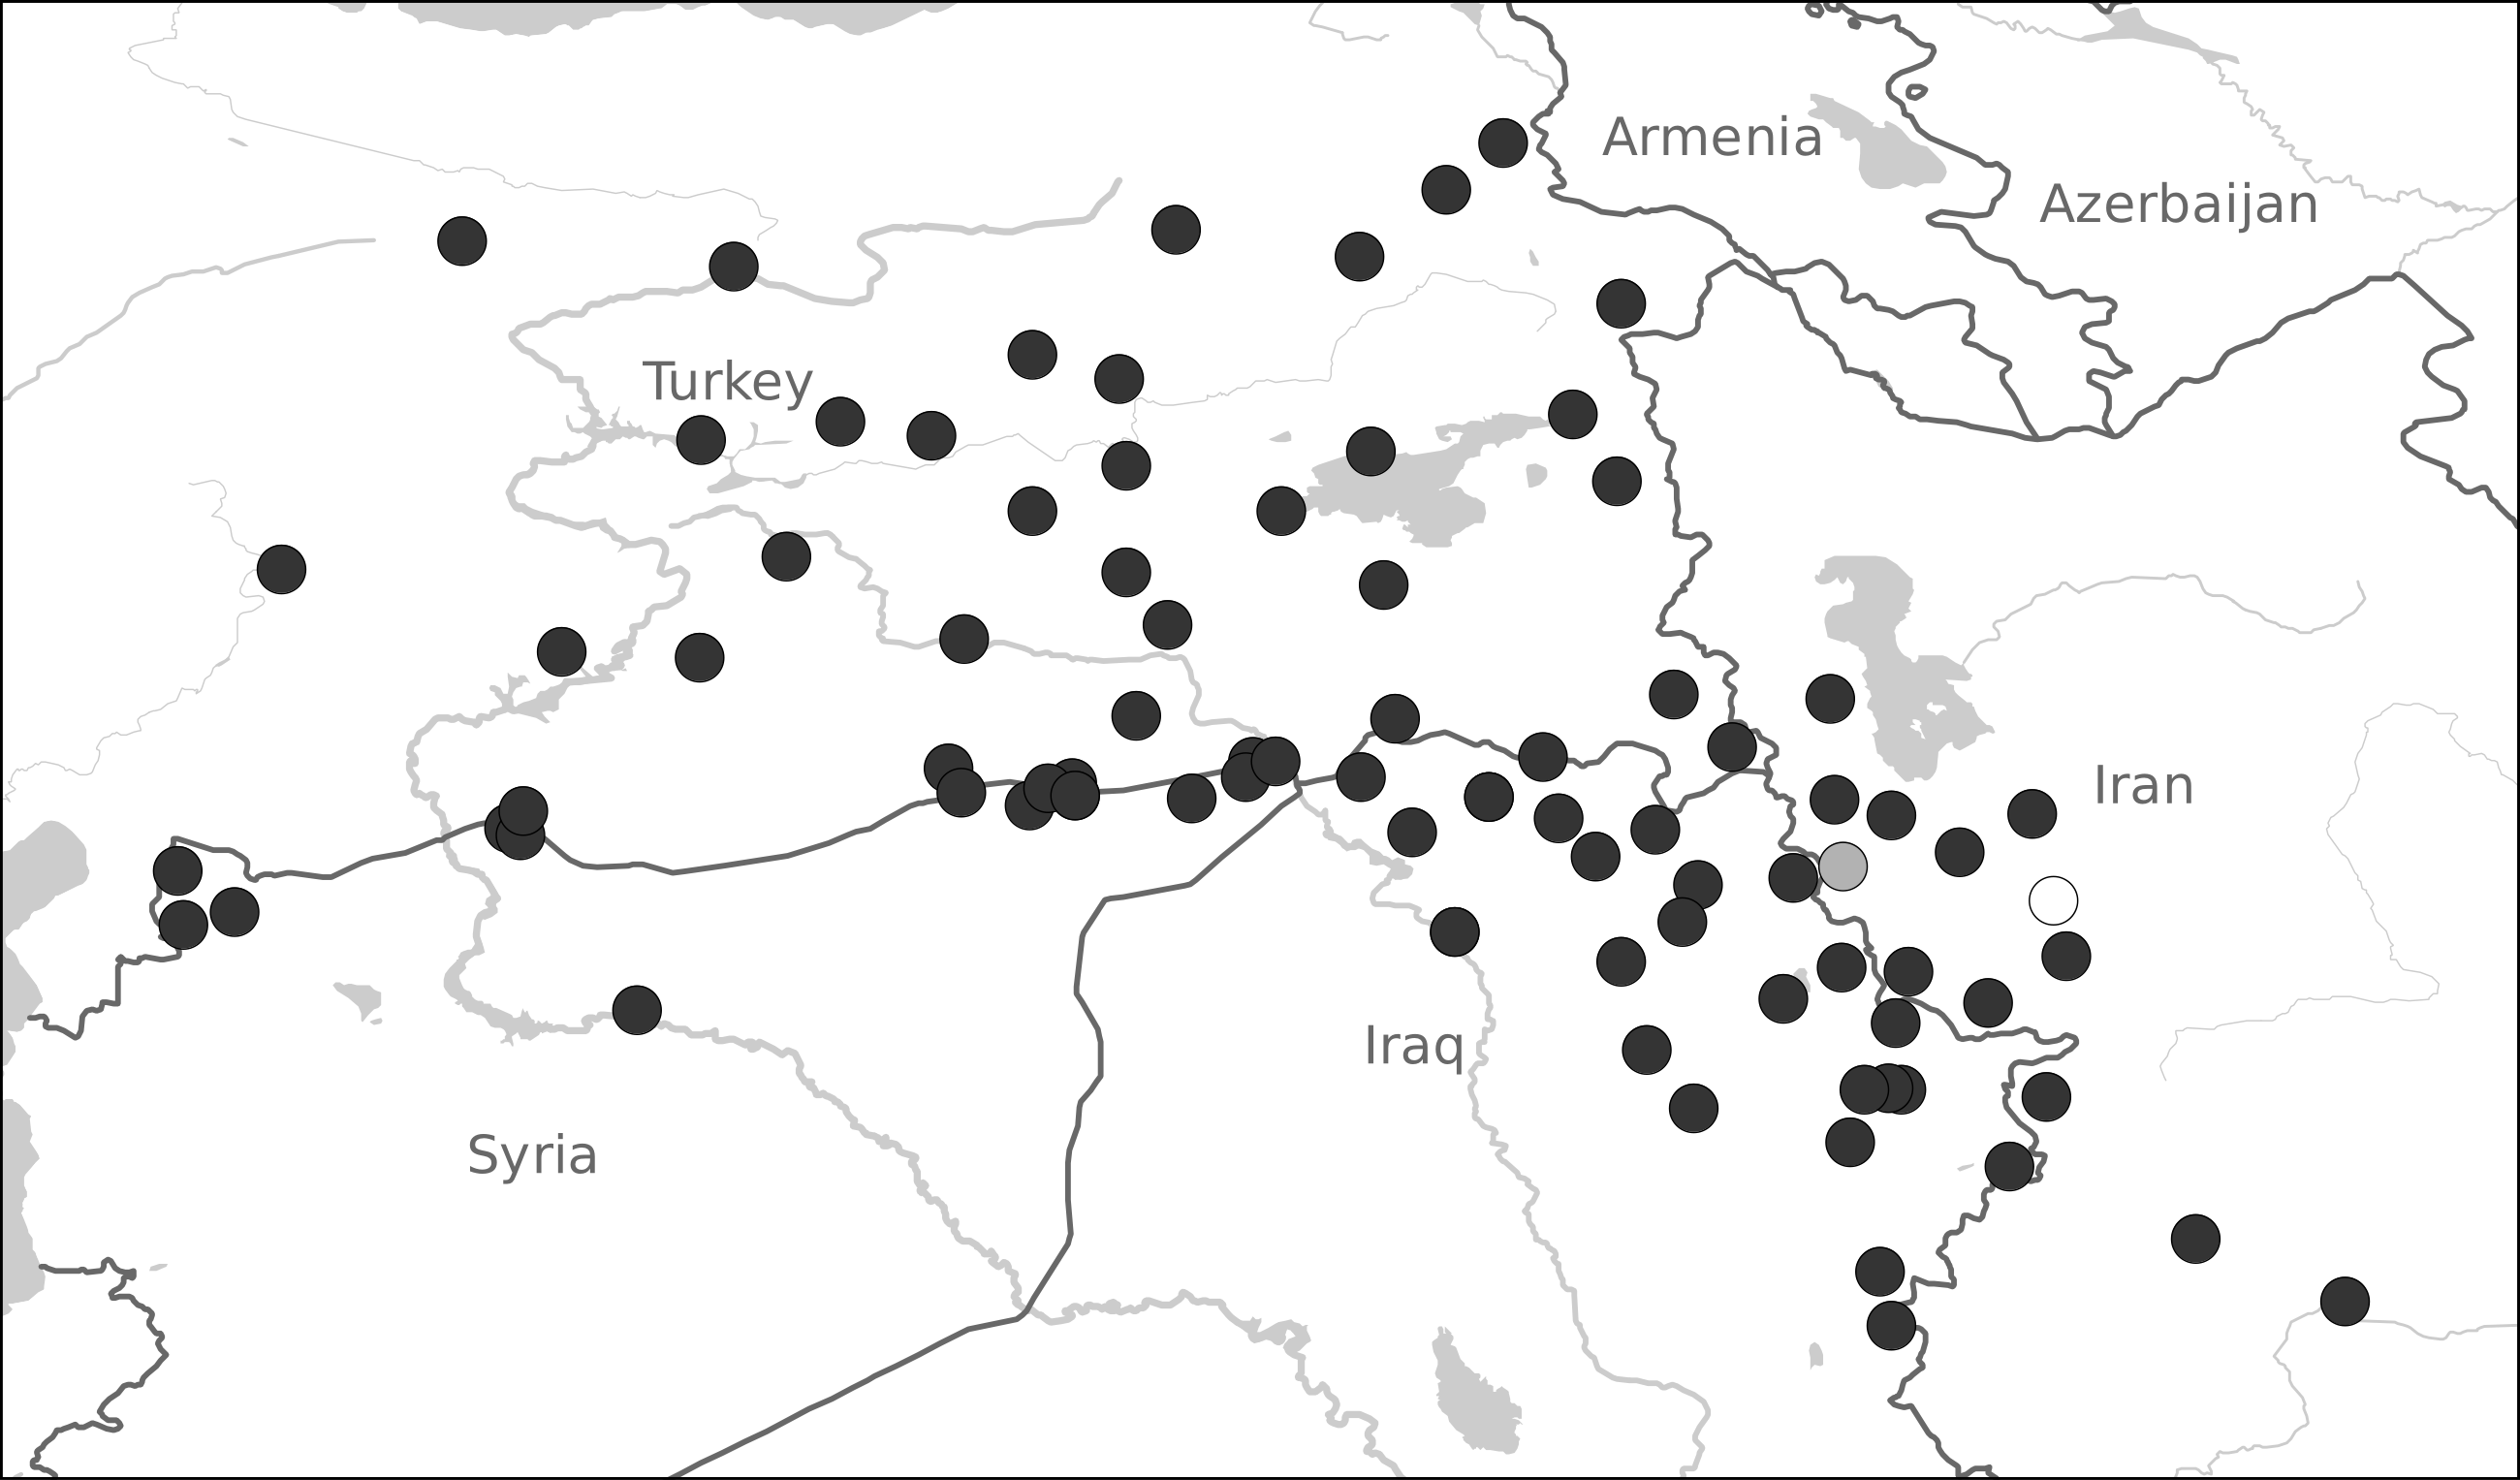
\includegraphics[width=\textwidth]{figures/fig3_map_motion.png}
\caption{\label{fig:key:2}Post-predicate goals of verbs of motion \citep[12]{Haig2022}}
\end{figure}

\begin{figure}
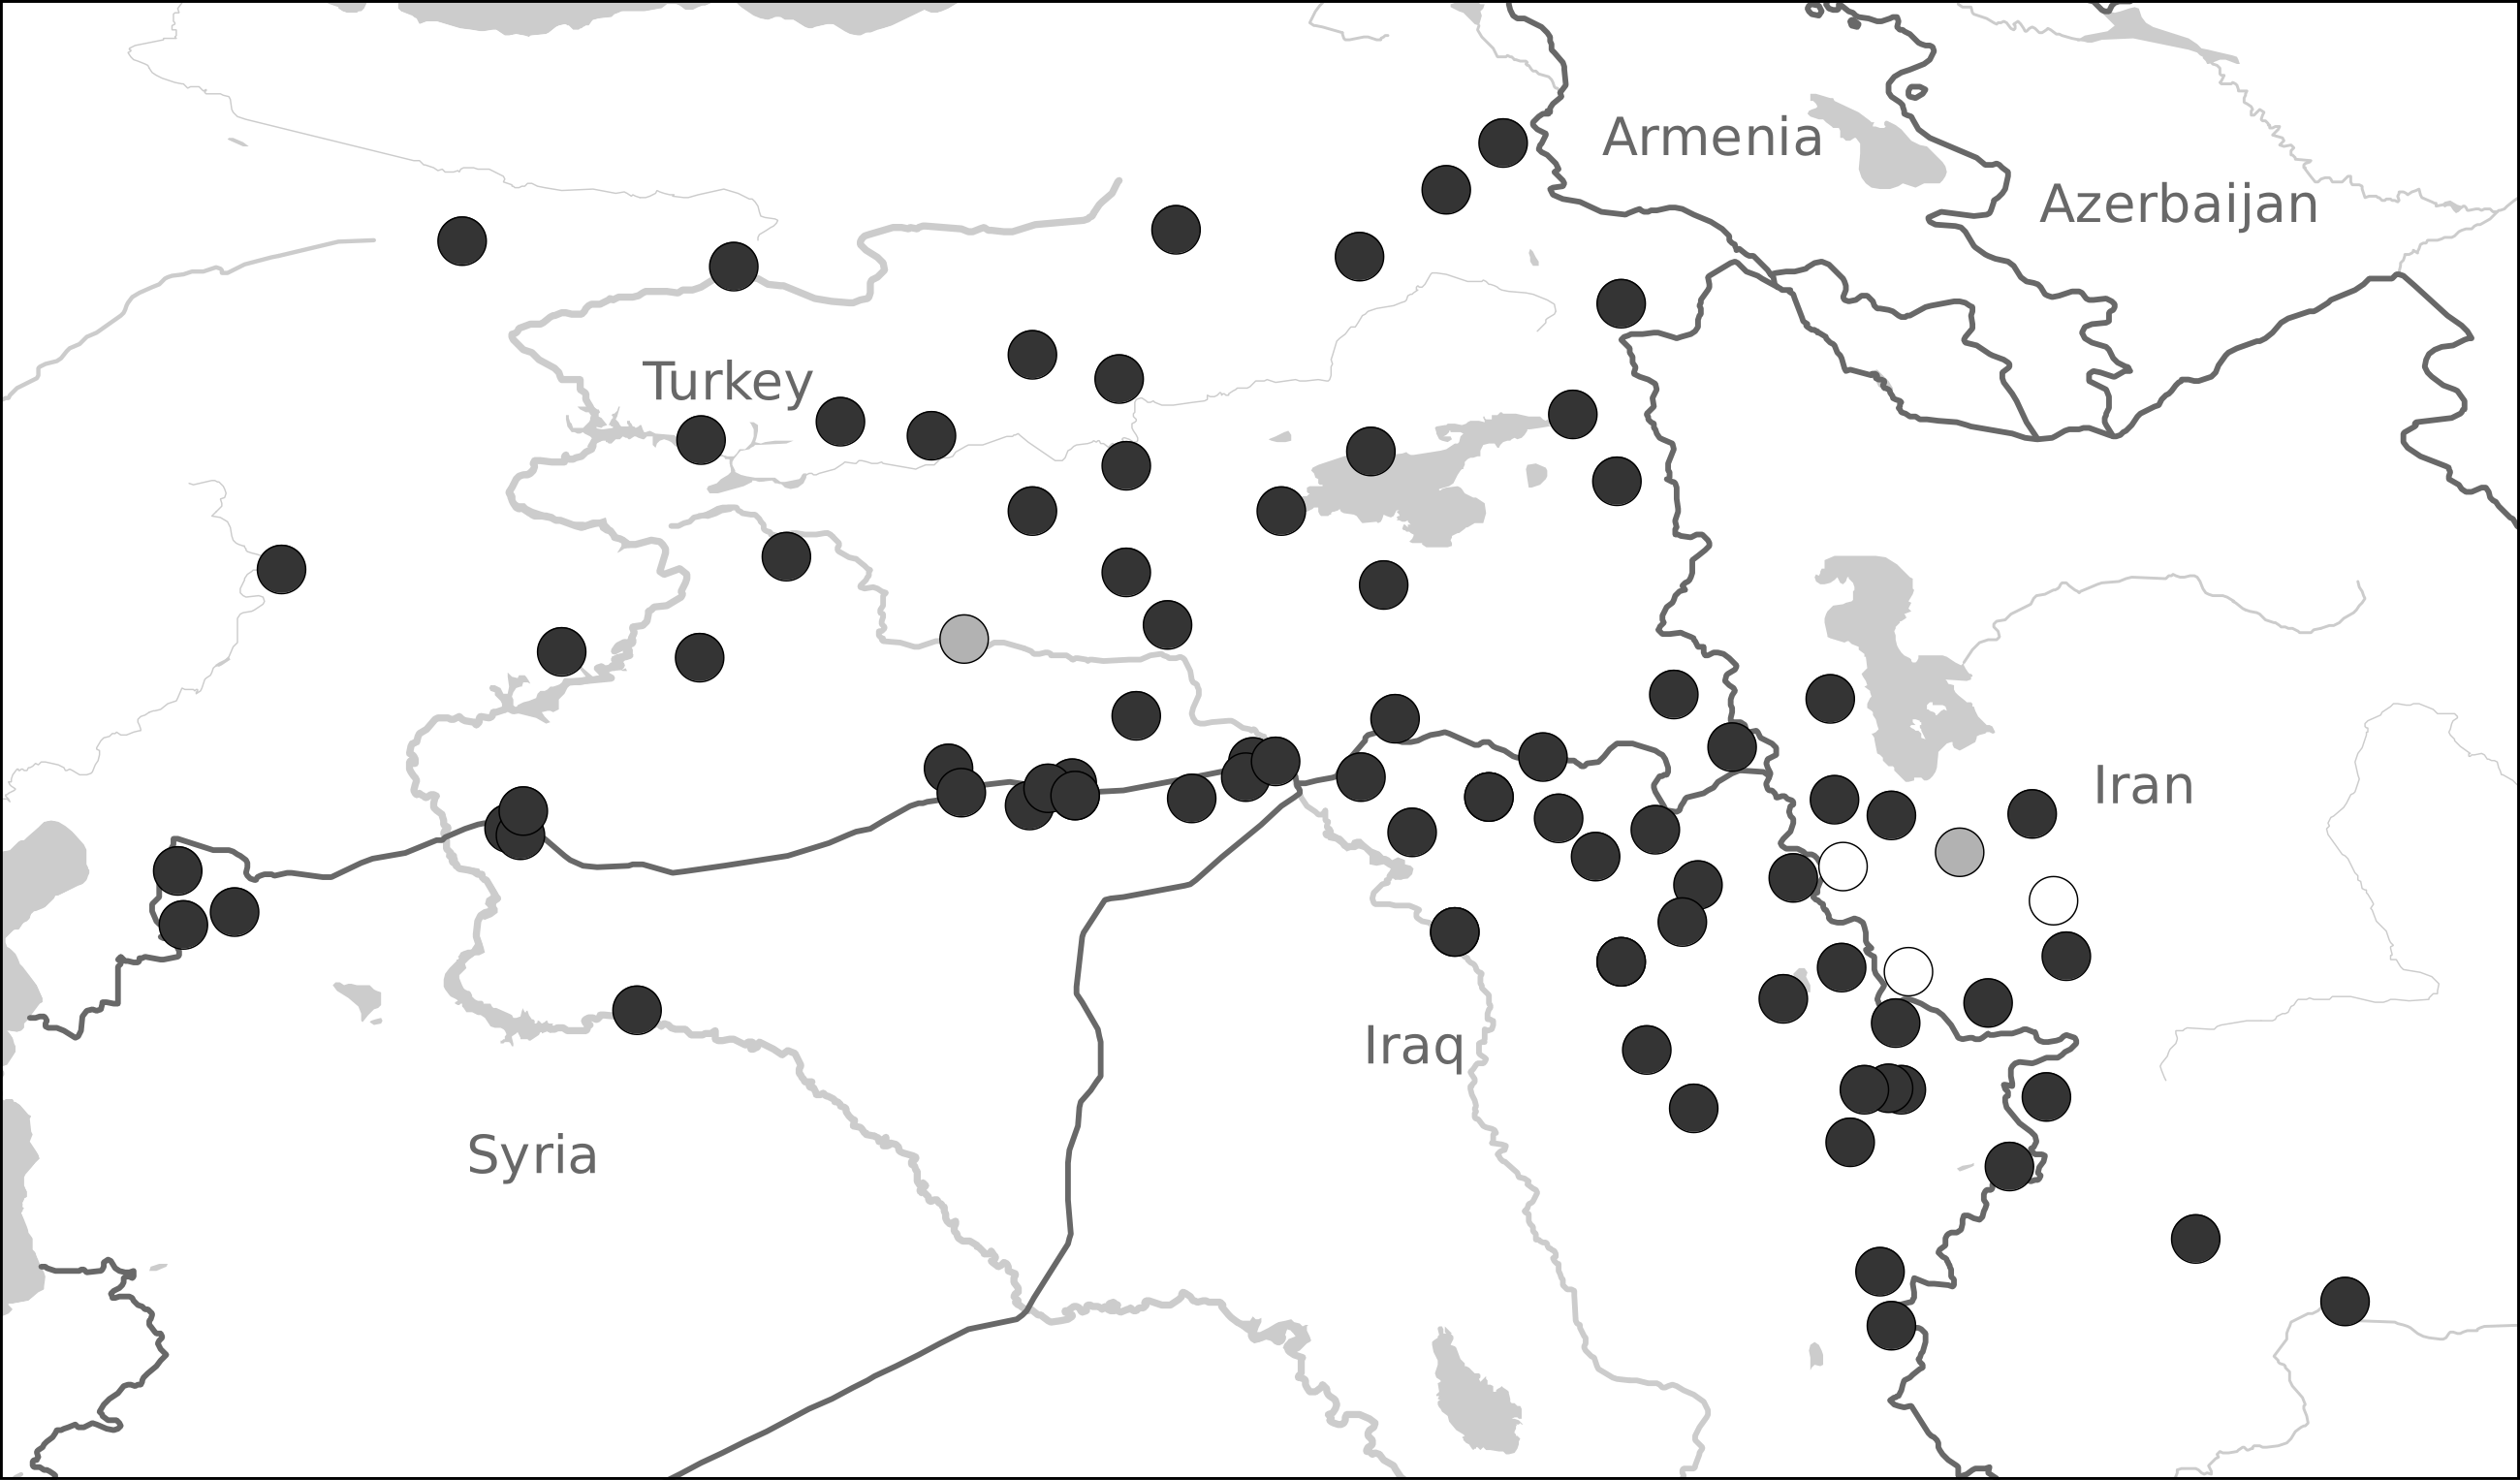
\includegraphics[width=\textwidth]{figures/fig4_map_causedmotion}
\caption{\label{fig:key:3}Post-predicate goals of verbs of caused motion \citep[12]{Haig2022}}
\end{figure}

Figures \ref{fig:key:2} and \ref{fig:key:3} illustrate the distribution of post-predicate goals for verbs of motion and caused motion across different Kurmanji dialects. Black dots indicate that at least 50\% of the goals were placed in the post-predicate position, while gray dots represent an equal number of goals placed in both the post- and pre-predicate positions. White dots indicate that less than 50\% of examples were positioned in the post-predicate position. It is important to note that the data encompass both types of flagging: goals flagged with adpositions as well as those flagged with case. Since case-flagged goals are always positioned post-predicatively, the figures do not provide a clear representation of the distribution of adpositional goals in the pre- and post-predicate positions. Furthermore, Figures \ref{fig:key:2} and \ref{fig:key:3} indicate that goals of motion and goals of caused motion are predominantly placed in the post-predicate position across all Kurmanji dialects. However, there are exceptions in the Kurmanji spoken in Iran, where pre-predicate goals make up the majority and are flagged with a preposition (for a discussion, see \citealt{Haig2022}: 13).

At the same time, \citet{Haig2014} observes that the use of post-predicate adpositional goals is quite limited in various Kurmanji dialects. In the southeastern Anatolian dialects, goals are frequently accompanied by a preposition or a circumposition. In contrast, the central Anatolian dialects do not use adpositions with goals, instead employing bare noun phrases (NPs). The only exception is for human goals, which are marked by the preposition \textit{cem} ‘to,’ as illustrated in example \REF{ex:key:17}.

\ea%17
  \label{ex:key:17} Kurmanji (\citealt{Matras2016}: K092, Sunak Köyü)\\
\gll Otobus     hat-e     cem   me \\
bus    come.\textsc{pst.3sg-drct}      \textsc{adp}    us\\
\glt ‘The bus came to us.’ 
  \z

The next type of goal are recipients of verbs of transfer. \citet{Haig2022} reports only two examples of goals of transfer in the Database of Kurdish Dialects, and both are flagged with case. Hence, the recipient argument in the examples is placed after the predicate.

\ea%18
  \label{ex:key:18} Kurmanji (\citealt{Matras2016}: K010, Tunceli)\\
  \gll Ew  ne-da      min \\
it  \textsc{neg-}give\textsc{.pst.3\textsc{sg}}  me\\
\glt ‘He didn’t give it to me.’ 
  \z

Furthermore, Gündoğdu (2019) notes that the semantics of verbs of transfer influence the flagging and positioning of their arguments. For instance, the verbs \textit{dan} ‘to give’ and \textit{firotin} ‘to sell’ flag their recipients with oblique case, resulting in these recipients being placed in the immediate post-predicate position. In contrast, the verb \textit{şandin} ‘to send’ flags its recipients with an adposition, placing them in the pre-predicate position.

The final type of goal is the addressees of verbs of speech. \figref{fig:key:4} illustrates the distribution of these goals in either the pre- or post-predicate position.

\begin{figure}
% 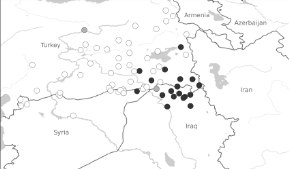
\includegraphics[width=\textwidth]{figures/iefremenko-img004.png}
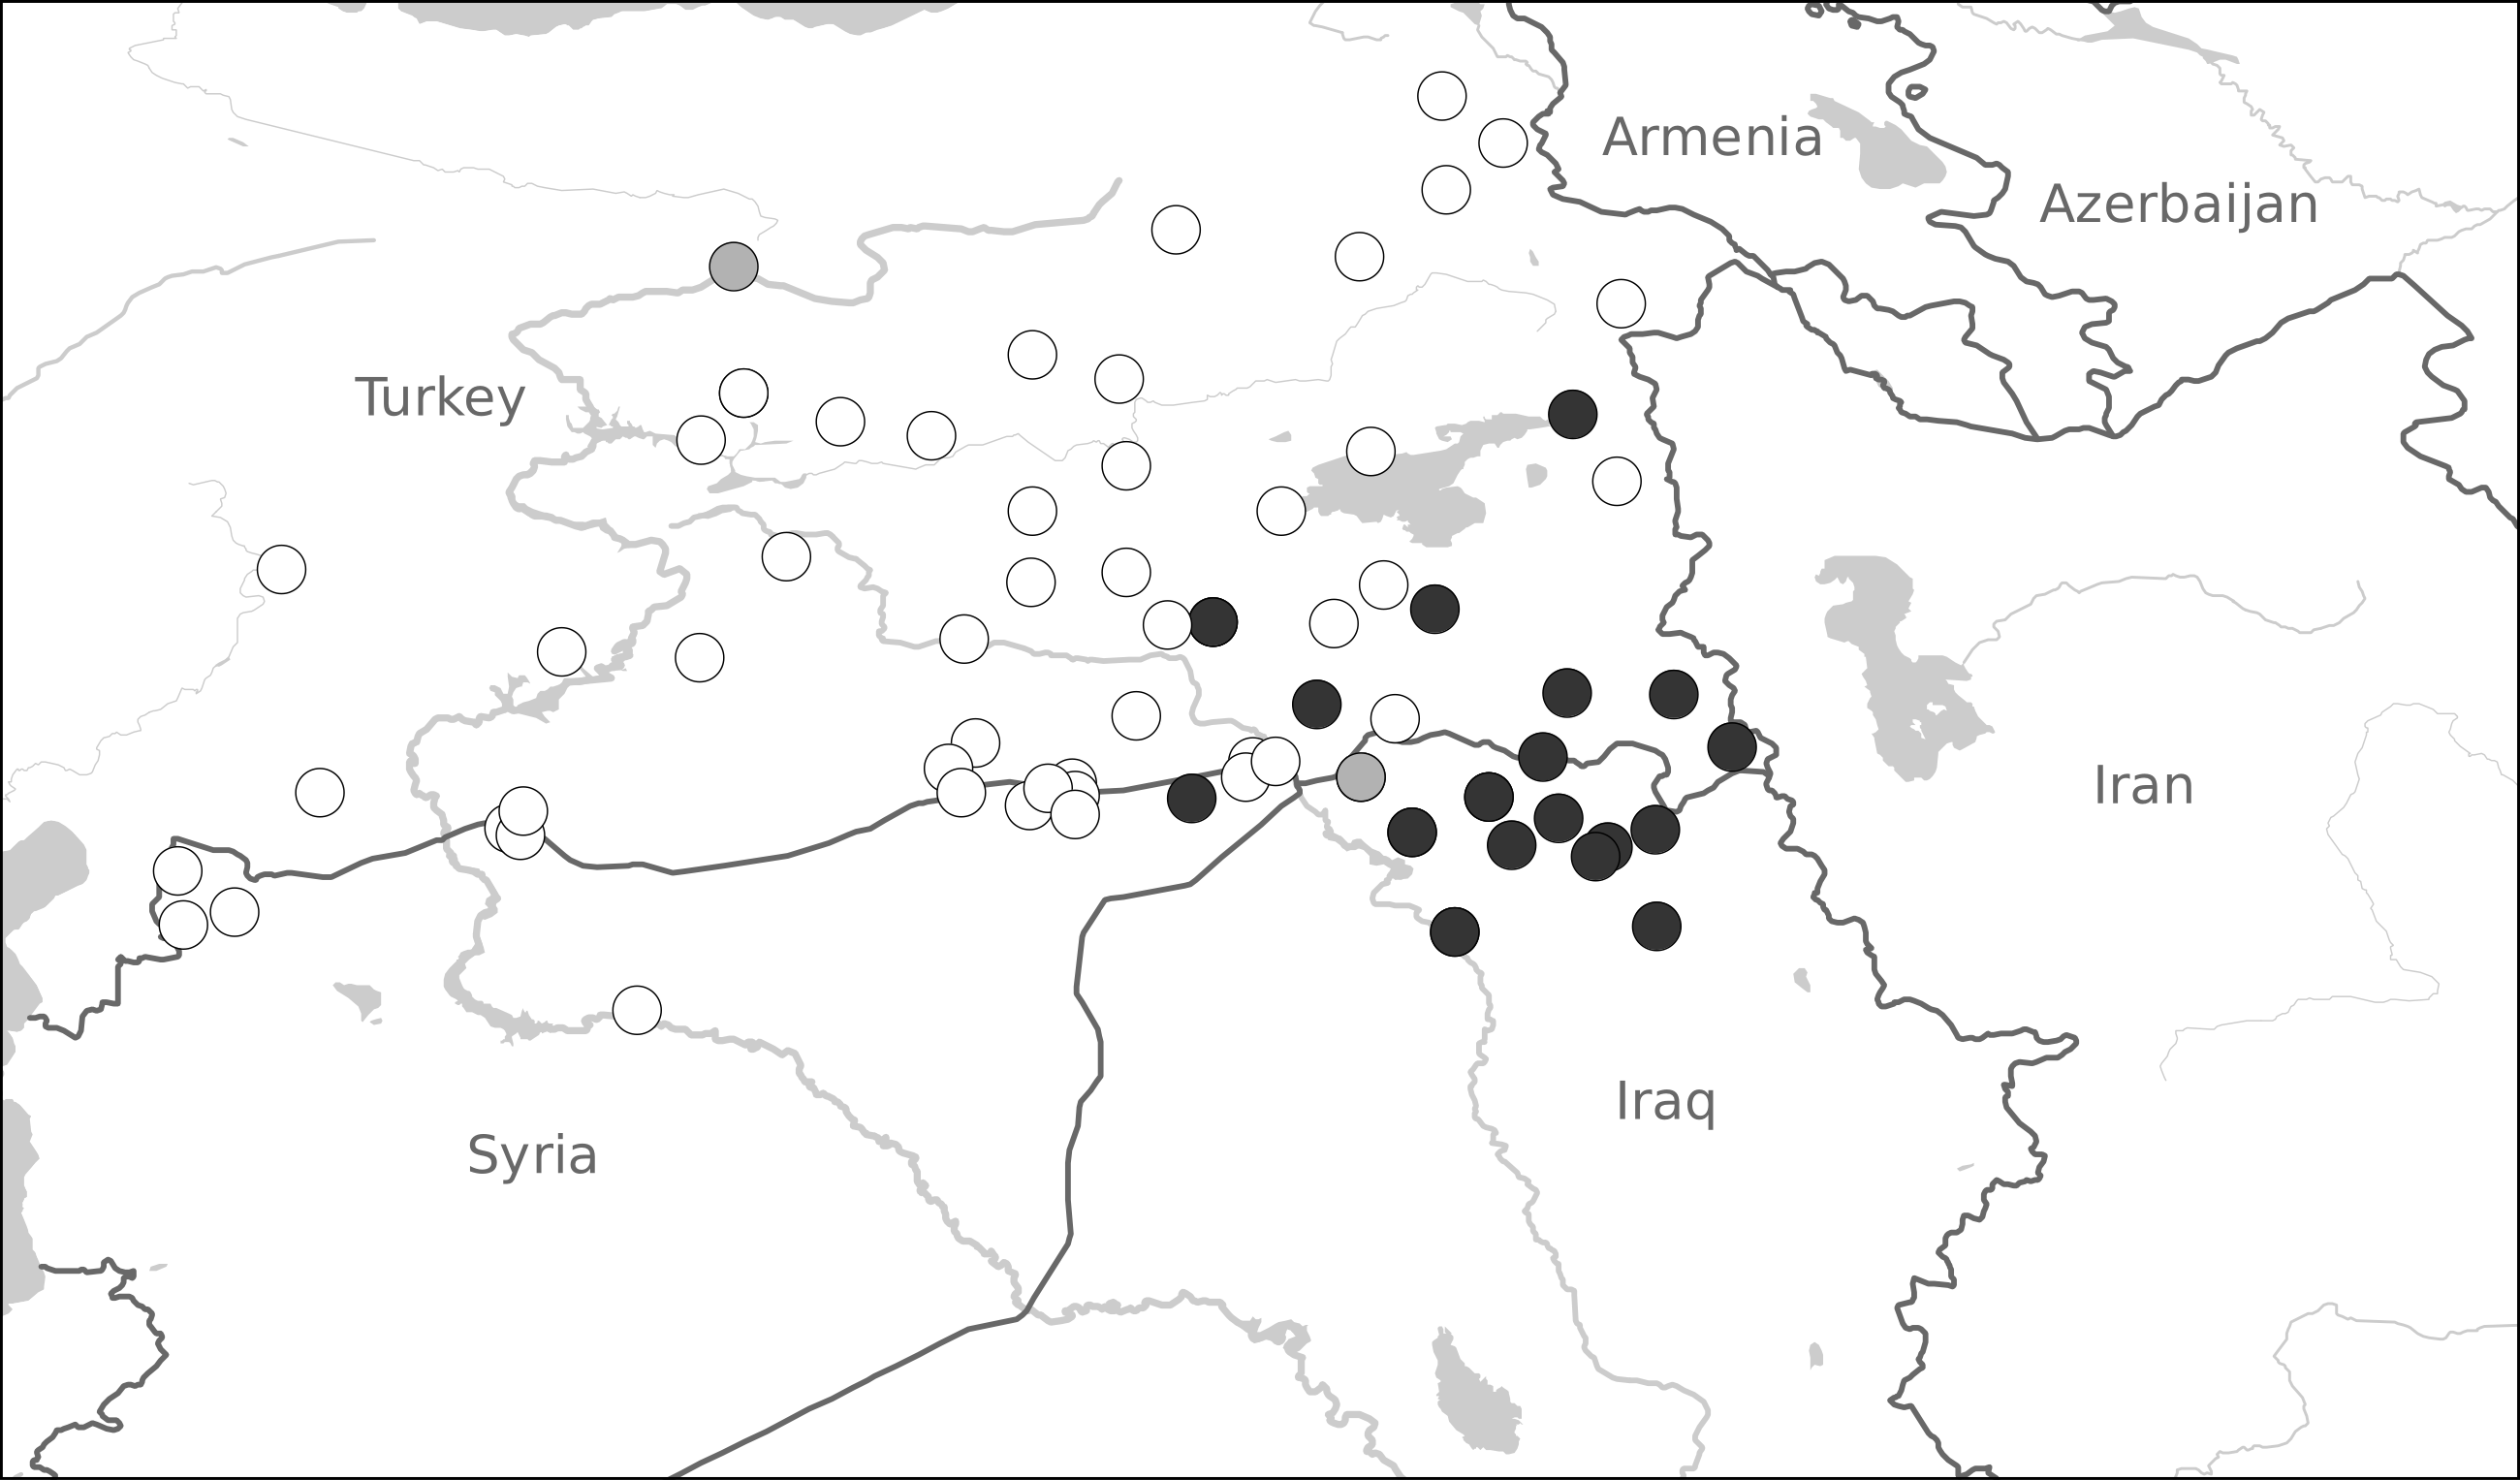
\includegraphics[width=\textwidth]{figures/fig5_map_addressee.png}
\caption{\label{fig:key:4}Post-predicate addressee arguments \citep[15]{Haig2022}.}
\end{figure}

\figref{fig:key:4} illustrates that in Kurmanji, addressees of verbs of speech are predominantly placed in the post-predicate position, particularly in southeastern Turkey and the Van province. In contrast, the northern dialects favor the pre-predicate position for addressees. For example, in Muş, the pre-predicate position for addressees of verbs of speech is a standard practice \citep{Haig2022}. As discussed by \citet{Haig2014}, the pre-predicate position for addressees is common in dialects that have developed circumpositions such as \textit{ji…ra} (e.g., Muş) or the independent postposition \textit{…ra} (e.g., Malatya). Thus, goal arguments introduced with circumpositions and postpositions are consistently placed in the pre-predicate position, while those flagged with prepositions are found in the post-predicate position (\citealt{Gundogdu2019}, \citealt{Haig2022}).

\citet{Haig2014} suggests that the variation observed among Kurmanji dialects can be attributed to language contact. This is particularly relevant given that Kurmanji is spoken in the Western Asian Transition Zone. The region can be understood as a contact zone between large-scale typological patterns, involving both differences in basic word order, namely (S)OV versus (S)VO, and differences in adpositional type, including prepositions, postpositions, and ambipositions (\citealt{HaigKhan2019}, \citealt{HaigEtAl2024}). Specifically, the OVX word order in Kurmanji developed through contact with earlier Semitic and Iranian languages (\citealt{Haig2014}, \citealt{HaigThiele2014}). Additionally, \citet{Haig2020} and \citet{Haignforth} note that in historically (S)OV languages, locational goals, along with recipients and addressees, are the primary candidates to move into the post-predicate position, while preverbal (indefinite) direct objects and copular complements tend to be more stable.

As a result of the aforementioned factors, the southernmost dialects, which have maintained prolonged contact with Neo-Aramaic, tend to place goals, addressees and recipients predominantly after the verb. In contrast, the northern and western dialects have experienced extensive contact with Armenian and Turkish, resulting in a strong preference for the preverbal placement of these constituents. Additionally, southern dialects show a tendency to use prepositions or circumpositions when introducing post-predicate elements. Conversely, in the dialects of Central Anatolia, the combination of a post-predicate consituent with a preposition is highly restricted.

\subsection{The effect of information structure on the use of the post-predicate position}\label{sec:key:3.3.3}

The placement of post-predicate elements in Kurmanji is syntactically fixed and is not affected by pragmatically driven scrambling or stylistic variation, in contrast to Turkish, for instance \citep{Haig2022}. As mentioned at the beginning of \sectref{sec:key:3.3}, this study focuses on Kurmanji as spoken in Turkey and Germany, while also drawing inspiration from research on other Kurdish languages and Persian.

\citet{Asadpour2021} conducted an extensive analysis of word order in goal constructions across various languages spoken in northwestern Iran, including Mukri Kurdish. This analysis examined multiple factors to provide a comprehensive understanding of word order patterns, including semantic factors such as animacy, number, and the semantic class of verbs. The author also investigated morphosyntactic factors, including part of speech, (in)definiteness, and flagging. Additionally, the analysis considered information structure as a discourse-pragmatic factor, along with the syntactic weight of constituents. The results indicated that the semantic class of verbs and flagging are significant predictors of the post-predicate position in Mukri Kurdish, aligning with findings from previous research on Kurmanji. However, Asadpour also demonstrated that information structure plays a crucial role in determining whether goals are placed in the pre- or post-predicate position in Mukri Kurdish. Specifically, it was found that goals in the pre-predicate position are primarily new and given-inactive, while those in the post-predicate position typically represent given or accessible information. This finding has not been previously documented in Kurdish, potentially due to the fact that Asadpour’s study focuses on Mukri Kurdish, which is spoken in northwestern Iran, whereas the studies discussed earlier primarily concentrate on Kurmanji spoken in Turkey. Considering that Kurdish languages are spoken across several countries and come into contact with various languages, the observed variations in these studies may stem from distinctions among the Kurdish languages.

Nevertheless, the current study will explore the influence of information structure on word order in Kurmanji, taking into account the findings from Mukri Kurdish as well as the role of information structure in the word order of Turkish, the contact language.

\subsection{The effect of formality and mode on the use of the post-predicate position} \label{sec:key:3.3.4}

Starting from the second half of the 20th century, efforts have been made to standardize the writing system for Kurmanji, using the Latin alphabet, with the grammar of \citet{KhanLescot1970} being one of the most significant contributions. However, the development of Kurmanji literacy has faced challenges due to social and political factors (\citealt{Derince2013}, \citealt{BrizicnodateEtAl}). In Turkey, Kurmanji speakers often achieve literacy in Turkish, and, in the best-case scenario, become acquainted with the written conventions of Kurmanji only in their adult years (\citealt{HaigMatras2002}). Additionally, Turkish serves as the sole language of governmental and educational institutions, while Kurmanji is primarily used in informal contexts. This lack of familiarity with written language norms of Kurmanji among the Kurmanji-speaking population in Turkey may explain why earlier studies on Kurmanji word order relied on spoken records. Consequently, the impact of mode or formality on word order in Kurmanji has remained largely unexplored.

However, examining Kurmanji's word order across different linguistic registers is important. One reason for this is that previous research on Persian, a language that shares syntactic features with other West Iranian languages, has identified a correlation between formality, mode, and word order. \citet{Frommer1981} found that in Persian, a lower degree of formality corresponds to an increase in post-predicate elements. In other words, while formal written registers are predominantly verb-final, informal spoken registers contain post-predicate elements in more than 70\% of utterances. Furthermore, a recent study by \citet{Haig_post-predicate_EtAl2024-1} supports the findings of \citet{Frommer1981}. By drawing parallels between Persian and Kurmanji, we can hypothesize that similar register effects may exist in Kurmanji, highlighting the need for systematic research on how formality and mode shape word order patterns in Kurmanji.

\section{Studies on the post-predicate position in Kurmanji in language contact situations} \label{sec:key:3.4}

For centuries, Kurds have lived in contact with speakers of various languages, including Persian, Arabic, Turkish, Armenian, and Neo-Aramaic, among others. These interactions have undoubtedly influenced the Kurdish language(s). However, language contact has not been the central focus in Iranian linguistics (\citealt{HaigMatras2002}). Recently, more linguists have begun to investigate the CLI on Kurmanji. Sections \ref{sec:key:2.2} and \ref{sec:key:2.3} provide an overview of several studies conducted in this area.

Contact-induced changes in word order, particularly in the post-predicate position, have attracted increasing interest among scholars in Kurdish linguistics. In addition to the previously mentioned studies (\citealt{Haig2014}, \citealt{Haig2018}, \citealt{Gundogdu2019} \citealt{Haig2022}, \citealt{Asadpour2021}), several other investigations have documented word order variation. For instance, \citet{Dorleijn1996} examined Kurmanji spoken in Diyarbakır, revealing that this dialect exhibits greater syntactic flexibility compared to other Kurmanji dialects. Specifically, speakers demonstrated a preference for using circumpositions to flag goals rather than relying solely on the oblique case. As a result, the placement of goals was not strictly limited to the post-predicate position. Furthermore, \citet{Mahalingappa2009} investigated the acquisition of ergativity in Kurmanji among children living in Kurdish villages near Erzurum. The findings revealed that these children predominantly adhered to the SOV word order pattern. Interestingly, while their parents also primarily produced SOV utterances, there were occasional instances in which subjects were positioned after the verb to emphasize their role, resulting in an OVS word order. In addition, \citet{Kirgiz2022} conducted a study on the acquisition of Kurmanji in bilingual children in Germany. Similar to Mahalingappa's findings, Kırgız found that the children predominantly followed a verb-final word order while placing case-flagged goals in the post-predicate position. Notably, some children also placed subjects in the post-predicate position, indicating a degree of flexibility in their use of word order. Finally, a study by \citet{Herkenrath2021} examines the use of post-predicate elements in three languages in contact: Kurmanji, Turkish, and German. The data were collected from monolingual, bilingual, and multilingual speakers who immigrated to Germany at different ages. The motivations for employing the post-predicate position vary across the three languages: predicate semantics in Kurmanji, information structure in Turkish, and syntactic structure in German. \citet{Herkenrath2021} notes that, in the language contact situations, the reasons for using the post-predicate position overlap among the languages, reflecting their mutual influence on one another. This exploratory study underscores the need for more in-depth investigations into the ongoing changes within these languages.

Studies on Kurmanji in contact situations show that while the language predominantly follows an SOV pattern, there is certain flexibility in the post-predicate position. Both child and adult speakers sometimes place subjects or other constituents after the verb for emphasis or pragmatic reasons. Contact with other languages, such as Turkish and German, further influences the use of post-predicate elements. However, existing studies are still limited in scope, and more systematic research is needed to fully understand how language contact shape word order in Kurmanji.

\section{Word order in German}\label{sec:key:3.5}

The basic word order in German is (S)OV with V2 features (\citealt{Fourquet1977}, \citealt{Bach1962}, \citealt{Bierwisch1966}, as stated in \citealt{kiss_41_2015}). SOV is typically exhibited in embedded and main clauses with periphrastic verb constructions. At the same time, the V2-constraint often leads to SVO or XVS orders in main clauses, as the finite verb is required to occupy the second position in the clause (\citealt{Czinglar2013, Czinglar2014}).

Given the various word order patterns in German, scholars have different opinions on the basic word order of German. Previous research suggests that the base word order in German is SOV. \citet{Muller2023} argues that the assumption of verb-final order as the base order is supported by several observations. For instance, in subordinate clauses introduced by conjunctions, the verb consistently appears in the final position, and verbs tend to cluster at the end of the sentence, as illustrated in example \REF{ex:key:19} below.

\ea%19
  \label{ex:key:19} German (\citealt{Muller2023}: 8) \\
\gll dass  er  ihn  gesehen  haben  muss \\
that  he  him  seen    have  must\\
\glt ‘that he must have seen him’ 
  \z

Secondly, verb particles form a close unit with the verb, and such units can be seen only in verb-final structures, as shown in the example \REF{ex:key:20a}. Consequently, this structure reflects the base order.

\ea \label{ex:key:20} German (\citealt{Muller2023}: 6) \\
\ea\label{ex:key:20a}
\gll weil    er  morgen  an-fängt\\
because  he  tomorrow  \textsc{prt}-start\\
\glt ‘Because he is starting tomorrow’
\ex\label{ex:key:20b}
\gll Er   fängt   morgen   an.\\
He  starts  tomorrow  \textsc{prt}\\
\glt   ‘He starts tomorrow.’ 
\z
\z

Furthermore, certain constructions allow only for (S)OV word order, such as verbs derived from nouns by back-formation (e.g., \textit{uraufführen} ‘to perform something for the first time’). As demonstrated in the examples \REF{ex:key:21} below, there is only one possible position for the verb.

\ea\label{ex:key:21} German (\citealt{Muller2023}: 137) \\
\ea[]{\label{ex:key:21a}
\gll weil     sie   das   Stück  heute  urauf-führen\\
because   they  the   play  today  \textsc{prt-}lead\\
\glt ‘because they are performing the play for the first time today.’
}
\ex[*]{\label{ex:key:21b}
\gll Sie  urauf-führen  heute  das   Stück.  \\
 they  \textsc{prt-}lead  today  the  play\\
 }
\ex[*]{\label{ex:key:21c}
\gll Sie  führen  heute  das  Stück  urauf.\\
they  lead  today  the  play  \textsc{prt} \\
}
\z
\z

Another example of the constructions that allow only SOV word order are verbs used together with the construction \textit{mehr als} ‘more than’ (see examples \REF{ex:key:22} below).

\ea \label{ex:key:22} German (\citealt{Muller2023}: 138) \\
\ea[]{\label{ex:key:22a}
\gll dass   Hans  seinen  Profit  letztes  Jahr  mehr  als  verdreifachte\\
that  Hans  his  profit  last  year  more  than  tripled\\
\glt ‘that Hans increased his profit last year by a factor greater than three.’
}
\ex[]{\label{ex:key:22b}
\gll Hans  hat   seinen   Profit   letztes   Jahr   mehr   als   verdreifact\\
Hans   has   his   profit   last   year   more   than   tripled\\
}
\glt ‘Hans increased his profit last year by a factor greater than three.’
\ex[*]{\label{ex:key:22c}
\gll Hans  verdreifachte  seinen Profit  letztes  Jahr  mehr  als\\
Hans  tripled    his  profit  last  year  more  than\\
}
\z
\z

Additional evidence for the base word order in German being (S)OV comes from the studies on the L1 acquisition of German that show that children start acquiring the word order with (S)OV structures (\citealt{ClahsenMuysken1986}, \citealt{Jordens1988}, \citealt{SchulzEtAl2008}, \citealt{TracyThoma2009}).

On the other hand, German is also characterized as a verb-second (V2) language. In German, V2 appears in main declarative clauses with a finite main verb, as shown in example \REF{ex:key:23}, and in wh-questions (\textit{W-Fragen}), as demonstrated in \REF{ex:key:24}. As for main declarative sentences with V2, any constituent can be placed before the finite verb \citep{Muller2023}, but importantly, only one constituent can be placed before the verb in the V2 word order \citep{Czinglar2013}. Although analyses of corpora of the spoken and written German language show that only half of the main sentences begin with a subject (\citealt{HinrichsKübler2005}, as cited in \citealt{Czinglar2013}), the existence of examples such as \REF{ex:key:23} and \REF{ex:key:24} has led some researchers to analyze German word order as SVO in main sentences and SOV in embedded clauses (for example, \citealt{Bohn1983}, as stated in \citealt{Vikner2019}) or as lacking a dominant word order altogether \citealt{wals-81}.

 \ea 
    \label{ex:key:23} German, self-constructed \\
 \gll Anna  schreibt  ihrem  Bruder    einen  Brief.\\
  Anna  writes    her  brother    a  letter\\
\glt ‘Anna is writing her a letter to her brother.’ 
\z

\ea%24
  \label{ex:key:24} German, self-constructed \\
\gll Was   schreibt Anna   ihrem   Bruder? \\
what  writes   Anna  her  brother\\
\glt ‘What is Anna writing to her brother?’ 
  \z

A widely used descriptive representation of German clause structure is provided by the Topological Model (\citealt{Drach1937}, \citealt{WollsteinEtAl2006}, \citealt{Wollstein-leisten2014, Wollstein2018}). As illustrated in \figref{fig:key:5}, finite and non-finite verbs together form a sentence bracket, which is positioned after the prefield and encompasses the middle field.


\begin{figure} 
\begin{tabular}{ccccc}
 & \multicolumn{3}{c}{$\overbrace{\hspace{7cm}}^{\text{\normalsize Sentence brackets}}$} & \\
Prefield & Left Bracket & Middle Field & Right Bracket & Postfield \\
\end{tabular}
\caption{\label{fig:key:5}Illustration of the Topological Model}
\end{figure}

In main clauses, the left bracket contains the finite verb, while the right bracket accommodates the infinite verb. The prefield allows for the fronting of any constituent, determined by discourse context and information structure, but the V2 constraint limits it to just one constituent. Furthermore, German can also place elements after the right bracket, and this construction is commonly referred to as \textit{Nachfeld} ‘post-field’ (\citealt{Frey2015}, \citealt{Hartmann2017}). The post-field is typically considered an area that holds heavy constituents, such as subordinate clauses or other constituents extraposed from the middle-field in order to reduce cognitive load (\citealt{Imo2015}, \citealt{Proske2015}). \tabref{tab:key:3.1} exemplifies the Topological Model for the German clause ‘(Yesterday we realized that) Maria (had) sent the child a letter from Berlin.’

\largerpage[3]
\begin{table}[b]\small
\begin{tabularx}{.95\textwidth}{llXlXlX}
\lsptoprule
\textbf{Prefield}  & \textbf{Left} & \textbf{Middle Field}  & \textbf{Right} & \textbf{Post-field}\\
& \textbf{Bracket} &  & \textbf{Bracket} & \\
\midrule
\textit{Maria} & \textit{schickte} & \textit{dem Kind einen Brief aus Berlin.} & &\\
Maria & sent & the child a letter from Berlin. &  & \\
\midrule
\textit{Maria} & \textit{hat} & \textit{dem Kind einen Brief} & \textit{geschickt} & \textit{aus Berlin.}\\
Maria & has & the child a letter & sent & from Berlin. \\
\midrule
\textit{Wir} & \textit{haben} & \textit{gestern} & \textit{festgestellt,} & \textit{dass Maria dem Kind einen Brief geschickt hat.} \\
We & have & yesterday & found out & that Maria had sent the child a letter from Berlin. &  \\
\lspbottomrule
\end{tabularx}
\caption{\label{tab:key:3.1} The Topological Model for German.}
\end{table}

As demonstrated in \tabref{tab:key:3.1}, the post-field can contain clausal (e.g., \textit{dass Maria dem Kind einen Brief geschickt hat} ‘that Maria had sent the child a letter’) or non-clausal constituents (\textit{aus Berlin} ‘from Berlin’). However, since the focus of this study lies in the non-clausal constituents positioned after the predicate, attention will be directed to them.

There are several types of non-clausal constituents placed in the post-field in German. Below are examples of such constituents, where \REF{ex:key:25} demonstrates an extraposed prepositional phrase, \REF{ex:key:26} shows an extraposed determiner phrase, \REF{ex:key:A} and \REF{ex:key:B} present an adverbial and an adjectival phrase respectively, and \REF{ex:key:C} is an example of a discourse marker in the post-field. Constituents that belong to the post-field in the examples (25-29) are in italics.

\ea%25
  \label{ex:key:25} German, (\citealt{Hartmann2017}: 101)\\
\gll Jeder    möge    seiner    Steuererklärung  ein Protestschreiben  beifügen,  \textit{mit} \textit{folgendem} \textit{Inhalt:} … \\
everybody  should    his    tax\_declaration  a protest\_letter    add    with  following  content …\\
\glt ‘Everybody should add a protest letter to his tax declaration with the following content.’ 
  \z

\ea%26
  \label{ex:key:26} German (\citealt{AkanHartmann2019}: 125)\\
\gll Auf  Gleis    eins  fährt  ein:  \textit{die} \textit{verspätete} \textit{Regionalbahn} \textit{nach} \textit{Wiesbaden.}\\
on  platform  one  arrives  \textsc{prt}  the  delayed  regional\_train to  Wiesbaden\\
\glt ‘The delayed train to Wiesbaden is arriving on platform one.’ 
  \z

Importantly, \citet{AkanHartmann2019} note that German allows only structurally complex determiner phrases in the post-predicate position, as in example \REF{ex:key:26}.

\ea%27
  \label{ex:key:A} German (\citealt{Frey2015}: 67)\\
\gll Wann  hat  Otto  gesprochen  mit  so  viel  Leidenschaft?  \\
  when  has  Otto  spoken    with  so  much  passion\\

  \gll Otto  hat  gesprochen  mit  so  viel  Leidenschaft  \textit{am} \textit{Montag}\\
Otto  has  spoken    with  so  much  passion  on  Monday\\
\glt --- ‘When did Otto speak with so much passion?’\\
     --- ‘Otto spoken with so much passion on Monday.’  \\
  \z
\newpage
\ea%28
  \label{ex:key:B} German, self-constructed\\
\gll Der  Kuchen  war  köstlich,  den  meine    Oma   gebacken  hat,  \textit{frisch} \textit{aus} \textit{dem} \textit{Ofen.}\\
 the  cake    was  delicious,  that  my    grandmother baked    has,  fresh  from  the  oven\\
\glt ‘The cake was delicious, which my grandmother baked, fresh out of the oven.’ 
  \z

\ea%29
  \label{ex:key:C} German (\citealt{Tsehaye2023}: 7) \\
\gll und   die  Autofahrer sind   dann   auch   gleich     ausgestiegen. \textit{und} \textit{so}\\
and  the drivers    are  then  also  immediately  exited    and  so on\\
\glt ‘And the drivers immediately exited and so on.’
  \z

Although the post-field has not received significant attention from researchers, some studies have investigated the use of constituents in the post-field. For instance, \citet{Proske2010}, as cited in \citet{Hartmann2017}, found that approximately one-third of the sentences in her data contain elements in the post-field, with 72\% of these instances being embedded clausal constituents. The remaining non-clausal elements in the post-field include prepositional phrases at 44\%, determiner phrases at 33\%, adverbials at 17\%, and adjectives at 6\%.

Furthermore, a recent study by \citet{Tsehaye2023} investigates the use of non-clausal constituents among monolingual adolescent German speakers in Germany and heritage speakers of German in the US, using data collected through the same methodology as that used in the current study. The findings indicate that 19.08\% of all utterances from monolingual speakers contained a non-clausal constituent in the post-field. Of these, 9.84\% were prepositional phrases, 5.02\% were discourse markers 2.01\% were adverbial phrases, 1.81\% were determiner phrases, and 0.4\% were adjectival phrases. Additionally, the study emphasizes that formality and mode significantly affect the production of non-clausal constituents in the post-field: speakers produced notably more post-field constituents in informal settings compared to formal ones, as well as in spoken mode rather than in written mode.

\largerpage
Other studies emphasize the impact of mode and formality on the use of the post-field in German. For example, \citegen{Engel1974} findings, as cited in \citet{Erdal1999}, indicate that extraposed elements occur five times more frequently in spoken data compared to written data. Similarly, \citet{Proske2015} notes that certain syntactic categories, such as specific adverbs and modal particles, appear in spoken language but are not acceptable in written texts. Conversely, \citet{Imo2015} does not address unacceptability but rather discusses different preferences for post-predicate constituents in spoken and written modes. Imo's research examines the occurrence of non-clausal constituents in the \textit{Nachfeld} in informal spoken and written settings. The findings reveal that the most common constituents in the \textit{Nachfeld} of spoken language are locative and temporal adverbs. However, the use of locative adverbs cannot be generalized as typical for the \textit{Nachfeld} in informal written German, instead, the temporal adverb \textit{heute} ‘today’ and various \textit{irgend}- ‘some-’ adverbs frequently appear. In addition to mode, formality also influences the use of the post-field in German. Previous research has documented significant variation in the frequency of post-field occurrences in written language, with the fewest instances found in scientific texts and the highest occurrences in informal productions (\citealt{Roelcke1997}, as cited in \citealt{Tsehaye2023}).

\section{Summary} \label{sec:key:3.6}

In summary, the word order in the three languages under investigation is SOV. However, each language employs the post-predicate position to different extents, influenced by different factors. Specifically, this position is determined by information structure in Turkish, predicate semantics in Kurmanji, and syntactic structure in German.

Despite these differences, there are also overlaps in the factors influencing the use of the post-predicate position. For example, \citet{Asadpour2021} suggests that, in addition to predicate semantics, information structure also affects the use of the post-predicate position in Kurdish, however, the data for this study are based on Mukri Kurdish spoken in Iran. If information structure similarly influences the word order of Kurmanji spoken in Turkey, it would indicate a shared factor—information structure—that affects both Kurmanji and Turkish in employing the post-predicate position.

Moreover, common factors influencing the use of the post-predicate position in Turkish and German include mode and formality: the post-predicate position tends to occur more frequently in spoken language compared to written language and in informal settings compared to formal ones. While the effects of formality and mode on word order in Kurmanji have not been thoroughly documented, some studies suggest these factors are relevant in Persian, a language that shares syntactic features with other West Iranian languages (\citealt{Frommer1981}, \citealt{Haig_post-predicate_EtAl2024-1}). The potential influence of formality and mode on the use of post-predicate constituents further emphasizes the importance of considering register as a factor in this analysis.

Ultimately, the combination of similarities and differences in the factors influencing the post-predicate position across Turkish, Kurmanji, and German makes this topic particularly intriguing for examination.

